The prefetcher is based on the report on itslearning named Managing Shared Resources in Chip Multiprocessor Memory Systems by Magnus Jahre. In order to predict
=======
\IEEEPARstart{T}{he} performance of a modern day microprocessor is much higher than that of typical memory. Much of the computational time is thus used to access the memory of the RAM and load it into the CPU. This is a growing bottleneck in a time where microprocessors are still increasing in performance. 
\\
\begin{figure}[h!]
	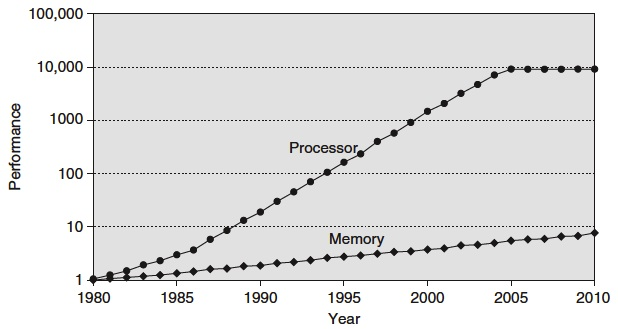
\includegraphics[scale = 0.5]{graphics/CPUmemoryGap.jpg}
	\caption{Dette er ei tekning}
\end{figure}
\\
A prefetcher reduces this bottleneck by predicting which instructions are addressed next. Memory fetches are attempted to be done before the memory is needed by the microprocessor, leading to a decreased time where the processor is stuck in a waiting state. If the prefetched memory addresses differ from what was needed, the processor needs to access the RAM anyway. This is the worst case scenario, in which the cache has no effect on performance.